\chapter{Authentication}
\label{ch:authentication}

\section{Product authentication}

\textbf{Status:} NOT APPLICABLE.

Expo Snips has no users, accounts, sessions or credentials of its own. It is a
local developer tool. A repository-wide inspection found no authentication code,
no token handling, no session storage, no OAuth client, no password logic and no
identity provider configuration in the product itself.

Consequences that follow directly from this:

\begin{itemize}
  \item The CLI requires no login and stores no credentials.
  \item The VS Code extension requires no login and stores no credentials.
  \item The registry is unauthenticated static hosting.
  \item \texttt{.expo-snips.json} contains no personal data.
  \item There is no MFA, no token lifecycle, no refresh flow and no session store
        to document. All of these are \textbf{NOT APPLICABLE}.
\end{itemize}

\section{Authentication templates generated for user applications}

The catalogue \emph{does} contain authentication \emph{screens}, which are
generated into the developer's own application. Those screens are not
authentication for Expo Snips; they are scaffolding for the developer's app.

The four auth recipes are:

\begin{longtable}{@{}L{3.6cm}L{1.5cm}L{1.9cm}L{7.4cm}@{}}
\caption{Authentication recipes}\\
\toprule
\textbf{Recipe} & \textbf{Version} & \textbf{UI} & \textbf{Generated files} \\
\midrule
\endfirsthead
\toprule
\textbf{Recipe} & \textbf{Version} & \textbf{UI} & \textbf{Generated files} \\
\midrule
\endhead
\texttt{auth/login} & 0.3.0 & native, shadcn & \texttt{app/login/index.tsx} (or
\texttt{screens/LoginScreen.tsx} for react-navigation),
\texttt{components/LoginForm.tsx}, \texttt{hooks/useLogin.ts|.js}; optional
\texttt{glass} variant. \\
\texttt{auth/register} & 0.2.0 & native, shadcn & \texttt{app/register/index.tsx} (or
\texttt{screens/RegisterScreen.tsx}), \texttt{components/RegisterForm.tsx},
\texttt{hooks/useRegister.ts|.js}. \\
\texttt{auth/forgot-password} & 0.2.0 & native, shadcn &
\texttt{app/forgot-password/index.tsx},
\texttt{components/ForgotPasswordForm.tsx}. \\
\texttt{auth/otp-verification} & 0.2.0 & native, shadcn &
\texttt{app/otp-verification/index.tsx}, \texttt{components/OtpInput.tsx}. \\
\bottomrule
\end{longtable}

\section{Validation model in generated screens}

All form-based auth recipes use the same pattern, implemented in the templates:

\begin{itemize}
  \item \texttt{react-hook-form} with the \texttt{Controller} component for
        controlled inputs;
  \item a \texttt{zod} schema and \texttt{zodResolver} for validation;
  \item a typed form data type derived with \texttt{z.infer<typeof schema>} in the
        TypeScript path, and an untyped equivalent in the JavaScript path;
  \item per-field error text rendered from \texttt{formState.errors}.
\end{itemize}

Example schema, reproduced from
\texttt{packages/registry/templates/auth/login/components.login-form.hbs}:

\begin{lstlisting}[language=JavaScript]
const schema = z.object({
  email: z.string().email('Invalid email address'),
  password: z.string().min(6, 'Password must be at least 6 characters'),
});

type FormData = z.infer<typeof schema>;
\end{lstlisting}

The shadcn variant uses slightly different messages
(\texttt{"Email is required"}, \texttt{"Enter a valid email"},
\texttt{"Password must be at least 6 characters"}).

\section{Authentication state and flow}

\begin{figure}[H]
\centering
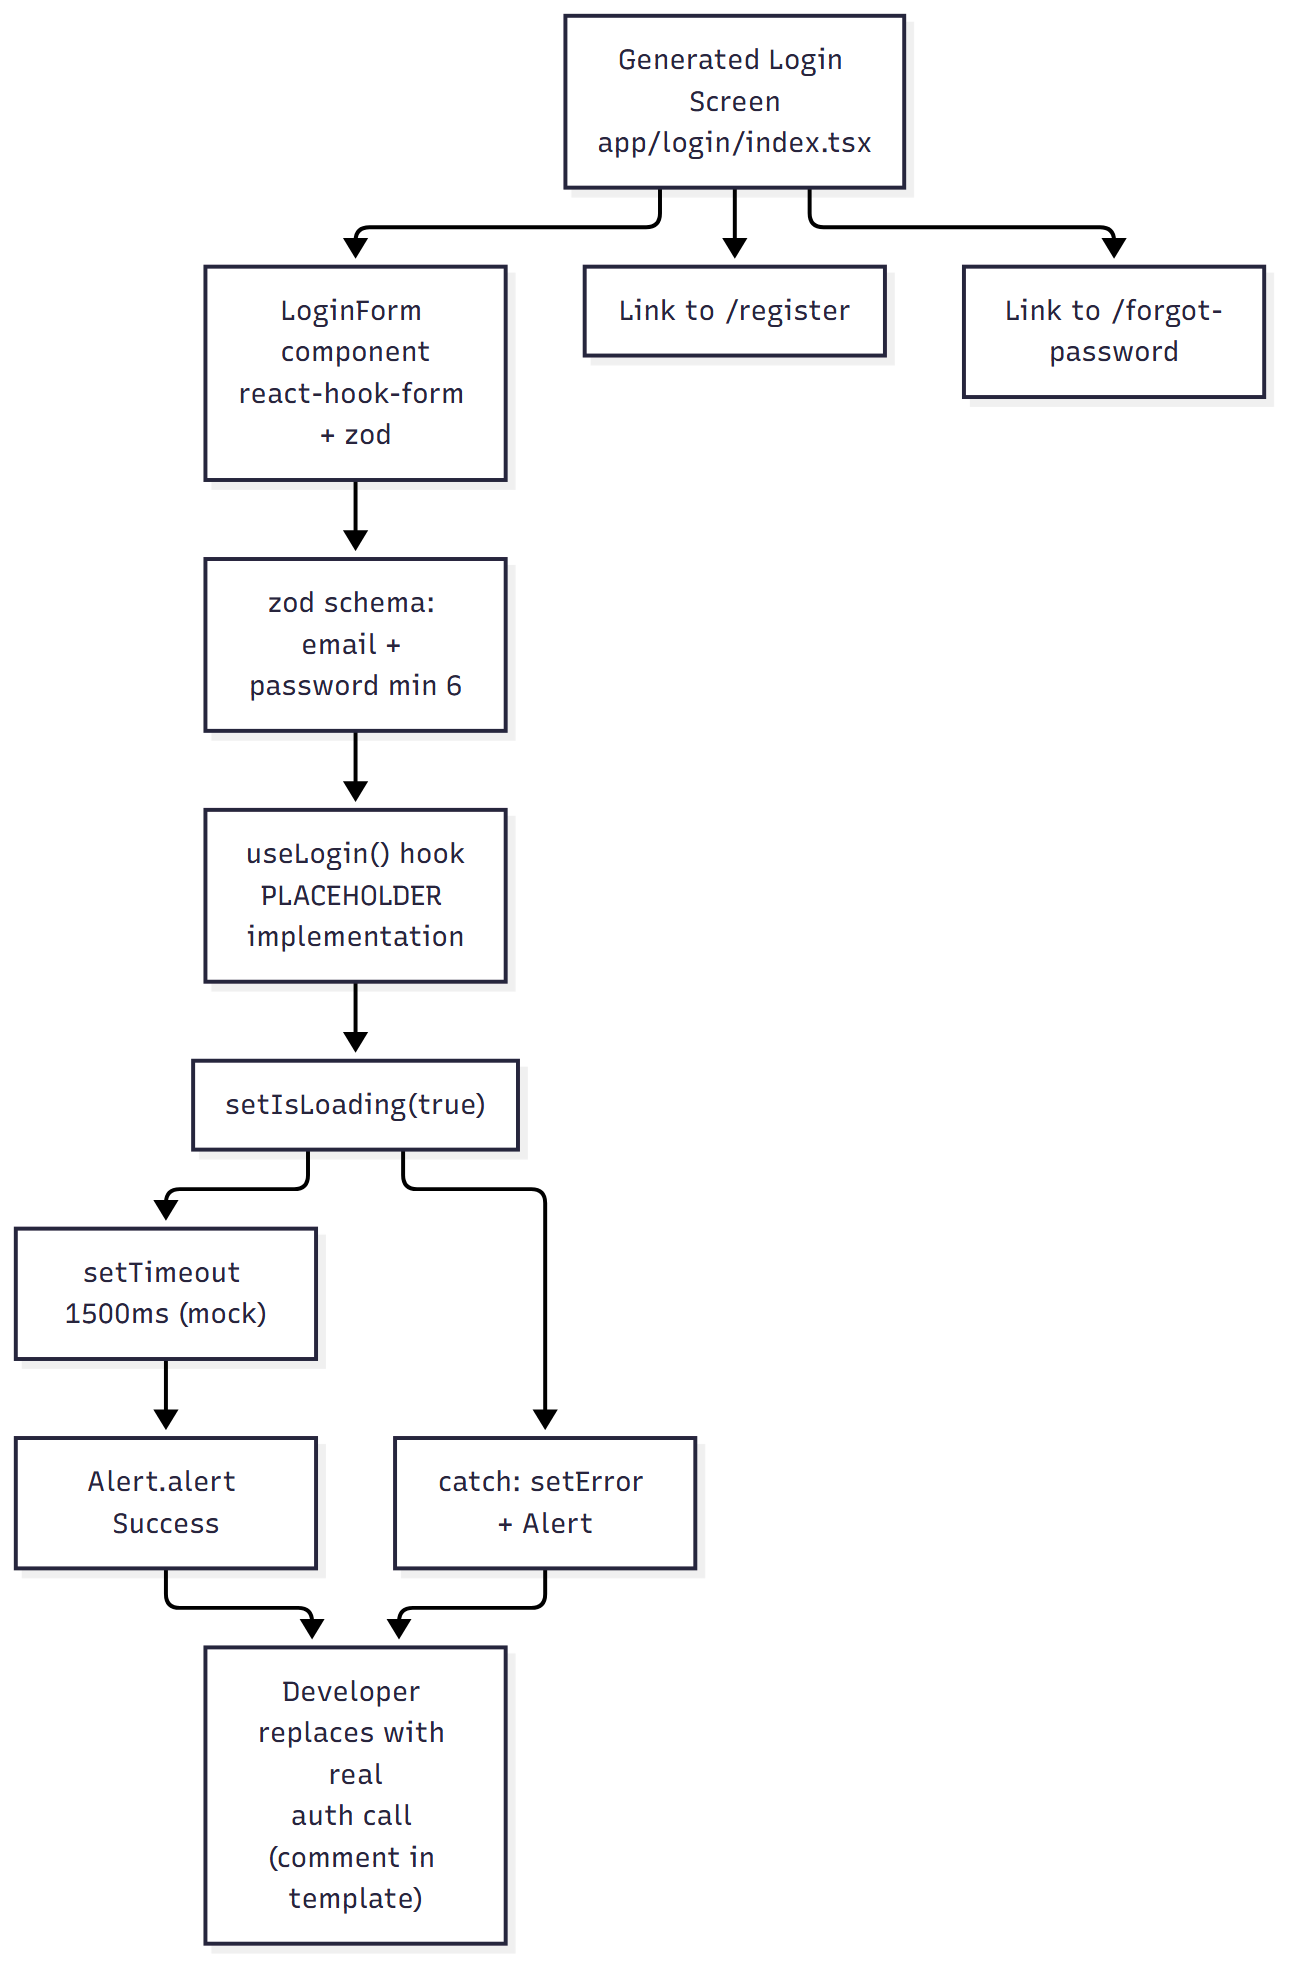
\includegraphics[width=0.78\textwidth]{diagrams/authentication-flow.png}
\caption{Authentication flow encoded in the generated templates (placeholder backend)}
\label{fig:authentication-flow}
\end{figure}

\textbf{Critical characteristic: the authentication backend is a placeholder.}
\texttt{hooks/use-login.hbs} and \texttt{hooks/use-register.hbs} implement:

\begin{itemize}
  \item \texttt{isLoading} and \texttt{error} state;
  \item a \texttt{console.log} of the submitted credentials;
  \item a mocked 1{,}500\,ms delay (\texttt{new Promise((resolve) =>
        setTimeout(resolve, 1500))});
  \item an \texttt{Alert.alert('Success', 'Logged in successfully')} on completion;
  \item a \texttt{catch} that stores the error message and shows an alert.
\end{itemize}

The template carries an explicit instruction to the developer:

\begin{lstlisting}[language=JavaScript]
// Replace with your actual authentication logic
// Example: await supabase.auth.signInWithPassword({ email, password });
\end{lstlisting}

\textbf{The shadcn variants differ materially.} The shadcn login form's
\texttt{onSubmit} simply runs \texttt{console.log(data)} --- it does not call the
\texttt{useLogin} hook at all
(\texttt{templates/auth/login/components.login-form.shadcn.hbs}). A developer
choosing \texttt{--ui shadcn} therefore receives a form with validation but no
loading or error handling from the hook. This inconsistency is recorded in
Chapter~\ref{ch:known-issues}.

\section{Password handling}

\begin{itemize}
  \item The native login form implements a secure-entry toggle: a
        \texttt{showPassword} state selects between \texttt{secureTextEntry} and an
        obscured/plain rendering, with \texttt{Eye}/\texttt{EyeOff} icons from
        \texttt{lucide-react-native}.
  \item The register recipe validates a password and a confirmation password with a
        \texttt{min(6)} rule.
  \item No password is ever persisted, hashed or transmitted by the product.
  \item The mocked hook logs the credentials to the console for demonstration; a
        developer should remove that \texttt{console.log} before shipping (see
        Chapter~\ref{ch:security}).
\end{itemize}

\textbf{Status:} IMPLEMENTED (templates) / RECOMMENDED (removing the console log).

\section{Session, token and MFA handling}

\textbf{Status:} NOT APPLICABLE.

No session storage, token issuance, refresh logic, secure storage, biometric flow,
or multi-factor authentication is present in the product, and none is generated by
default. The OTP recipe provides a one-time-code \emph{input experience}
(\texttt{components/OtpInput.tsx} with auto-advance behaviour) but contains no code
verification backend; the developer must supply that. The
\texttt{auth/otp-verification} recipe depends only on
\texttt{lucide-react-native}.

\section{Recommendations for users of the generated auth screens}

\begin{itemize}
  \item Replace the mock \texttt{useLogin}/\texttt{useRegister} bodies with a real
        authentication call (the templates suggest Supabase as an example only).
  \item Remove the credential \texttt{console.log}.
  \item Add secure storage (for example \texttt{expo-secure-store}) for any
        session token --- the templates do not include one.
  \item Wire navigation to the real post-login route; templates link to
        \texttt{/register} and \texttt{/forgot-password} by convention and do not
        perform authentication redirects.
\end{itemize}

\textbf{Status:} RECOMMENDED.
